\documentclass[boxes, qed]{homework}
\usepackage{xcolor,amsmath,listings}
\usepackage{graphicx}
\usepackage[backend=biber, style=mla, citestyle=authoryear]{biblatex}

\addbibresource{homework-9.bib}
\graphicspath{ {./images/} }

\name{Rohit Wason}
\course{Math 560}
\term{Spring 2021}
\hwnum{(\#9, Inference of Two-Way Tables)}

\newcommand{\bigzero}{\mbox{\normalfont\Large\bfseries 0}}
\newcommand{\rvline}{\hspace*{-\arraycolsep}\vline\hspace*{-\arraycolsep}}

\begin{document}

\begin{problem}
  A table of two-variables is given:\\
 
  \begin{tabular}{l|l|l|l}
    \hline
    Coffee & Male & Female & Total \\
    \hline
    Always &    $18$ & $15$ & $33$ \\
    Sometimes & $36$ & $36$ & $72$ \\
    Never &     $36$ & $9$ &  $45$ \\
    \hline
    Total &     $90$ & $60$ & $150$ \\
    \hline
  \end{tabular}\\
\end{problem}
\begin{solution}
  The expected cell counts are as follows:\\

  \begin{tabular}{l|l|l}
    \hline
    Coffee & Male & Female \\
    \hline
    Always &    $\frac{33\times 90}{150}=19.8$ & $\frac{33\times 60}{150}=13.2$ \\
    Sometimes & $\frac{72\times 90}{150}=43.2$ & $\frac{72\times 60}{150}=28.8$ \\
    Never &     $\frac{45\times 90}{150}=27$ & $\frac{45\times 60}{150}=18$ \\
    \hline
  \end{tabular}\\

  \textbf{Hypothesis}: $H_0$: There is no association between the row \& the column variables vs.
  $H_a$: There is an association between them. \\

  \textbf{The test statistic}, $\chi^2$
  \begin{align*}
    &=\sum{\frac{(\mathrm{observed\ count}-\mathrm{expected\ count})^2}{\mathrm{expected\ count}}}\\
    &=\frac{(18-19.8)^2}{19.8} 
    +\frac{(15-13.2)^2}{13.2} 
    +\frac{(36-43.2)^2}{43.2} 
    +\frac{(36-28.8)^2}{28.8}
    +\frac{(36-27)^2}{27}
    +\frac{(9-18)^2}{18}\\
    &=0.1636364+0.2454545+1.2+1.8+3+4.5\\
    &=10.90909
  \end{align*}

  Looking up the \textit{$\chi^2$ distribution critical values} table, we see that
  the \textbf{Critical value} at $\alpha=0.01$ and
  with \textbf{Degrees of freedom}, $df=(r-1)(c-1)=2$ comes out to be,
  $\chi^{2*}=4.605$.\\

  \textbf{Conclusion:}
  Since $\chi^2>\chi^{2*}$ we \textbf{reject} the hypothesis $H_0$, that there 
  is no association between the coffee consumption \& gender of the students.
\end{solution}

\begin{problem}
  Given\\

  \begin{tabular}{|l|l|l|l|l|l|l|}
    \hline
    Outcome & 1 & 2 & 3 & 4 & 5 & 6 \\
    \hline
    \# of occurances & $153$ & $184$ & $160$ & $175$ & $162$ & $166$ \\
    \hline
  \end{tabular}\\
\end{problem}
\begin{solution}
  We are to perform a Goodness of Fit test at $\alpha=0.05$ that the 
  die is fair.\\

  \textbf{Hypothesis}: $H_0$: The outcome from this die follows a fair distribution (where
  each outcome is $\frac{1}{6}$ likely) vs.
  $H_a$: The die is not fair. \\

  The \textbf{expected counts} for a fair die, when rolled $1000$ times would be $\approx 166.67$ \\

  \textbf{The test statistic}, $\chi^2$
  \begin{align*}
    &=\sum{\frac{(\mathrm{observed\ count}-\mathrm{expected\ count})^2}{\mathrm{expected\ count}}}\\
    &=\frac{1}{166.67} [
      (153-166.67)^2 
      +(184-166.67)^2
      +(160-166.67)^2 \\
      &+(175-166.67)^2 
      +(162-166.67)^2  
      +(166-166.67)^2 ]\\
    & \approx 3.739926
  \end{align*}

  Looking up the \textit{$\chi^2$ distribution critical values} table, we see that
  the \textbf{Critical value} at $\alpha=0.05$ and
  with \textbf{Degrees of freedom}, $df=(k-1)=5$ comes out to be,
  $\chi^{2*}=11.070$.\\

  \textbf{Conclusion:}
  Since $\chi^2<\chi^{2*}$ we \textbf{fail to reject} the hypothesis $H_0$, that this
  is a fair die.
\end{solution}

\begin{problem}Given:\\
  $n=500$\\
  Mean height of the fathers, $\bar{x}=67.9$\\
  Standard deviation of the height of fathers, $s_x=2.75$\\
  Mean height of the sons, $\bar{y}=68.7$\\
  Standard deviation of the height of sons, $s_y=2.83$
\end{problem}
\begin{solution}
  (a) The correlation between the heights of the sons and their fathers in the sample was $r=0.5$.
    The equation of the least-squares regression line for predicting the height of a son ($y$) from this 
    population based on his father’s height ($x$) is given by
    $$\hat{y}=b_0+b_1x$$
    where $b_1=r(s_y/s_x) = 0.5(\frac{2.83}{2.75}) \approx 0.5145$ \\
    and $b_0=\bar{y}-b_1\bar{x} = 68.7-0.5145(67.9) \approx 33.7654$\\
    
    Therefore the equation of the least squares regression line is
    \begin{equation}
      \hat{y}=33.7654+0.5145x
    \end{equation}
    
  (b) Suppose instead that the correlation was $1$. In this case the equation of the least-squares
    regression line for predicting the height of a son from this population based on his father’s height
    will use $b_1=s_y/s_x = \frac{2.83}{2.75} \approx 1.0291$ \\
    and $b_0=\bar{y}-b_1\bar{x} = 68.7-1.0291(67.9) \approx -1.1759$\\
    
    Therefore the equation of the least squares regression line will be
    \begin{equation}
      \hat{y} = -1.1759 + 1.0291x
    \end{equation}
    
  (c) If, instead, the correlation was $0$. $b_1=0(s_y/s_x) = 0$ \\
    and $b_0=\bar{y}-b_1\bar{x} = 68.7-0 = 68.7$\\

    This time, the equation of the least squares regression line will be
    \begin{equation}
      \hat{y} = 68.7
    \end{equation}

  (d) Predicting the height of a son from this population whose father is 6 feet 6 inches tall ($x=78$)
  based on the regression line obtained in (3.1) will be
  $$\hat{y} = 33.7654+0.5145(78) = 73.8964$$
  Or approximately 6 feet 2 inches.\\
  
  (e) If r was equal to $1$, using (3.2),
  $$\hat{y}(x=78) = -1.1759 + 1.0291(78) \approx 79.0939$$
  Or approximately 6 feet 7 inches.\\
  
  (f) And finally, if r was equal to $0$, using (3.3),
  $$\hat{y}(x=78) = 68.7$$
  Or approximately 5 feet 9 inches.
\end{solution}

\pagebreak

\section*{Project details}
\subsection*{Introduction}
According to the World Health Organization (WHO) stroke is the 2nd leading cause of death globally, 
responsible for approximately 11\% of total deaths. This dataset is used to predict whether a patient
is likely to get stroke based on the input parameters like gender, age, various diseases, and smoking 
status. We can use this dataset to state hypotheses of correlation between various explanatory
variables (like, age, bmi, marital status, residence type, etc.) and the result that they have had
a stroke.\\
The dataset used here can be found on Kaggle, a public competetion forum
where data scientists and novices collaborate to find answers in complex datasets
(\cite{kaggle}). This dataset contains $5110$ data points with $12$ variables:
\begin{enumerate}
  \item \textbf{id:} unique identifier
  \item \textbf{gender:} "Male", "Female" or "Other"
  \item \textbf{age:} age of the patient
  \item \textbf{hypertension:} 0 if the patient doesn't have hypertension, 1 if the patient has hypertension
  \item \textbf{heart\_disease:} 0 if the patient doesn't have any heart diseases, 1 if the patient has a heart disease
  \item \textbf{ever\_married:} ``No'' or ``Yes''
  \item \textbf{work\_type:} ``children'', ``Govt\_jov'', ``Never\_worked'', ``Private'' or ``Self-employed''
  \item \textbf{Residence\_type:} "Rural" or "Urban"
  \item \textbf{avg\_glucose\_level:} average glucose level in blood
  \item \textbf{bmi:} body mass index
  \item \textbf{smoking\_status:} "formerly smoked", "never smoked", "smokes" or "Unknown"*
  \item \textbf{stroke:} 1 if the patient had a stroke or 0 if not
\end{enumerate}

\subsection*{Methods}
According to stroke.org, a non-profit organization dedicated to public awareness about,
and prevention of common causes of stroke, smoking, lack of physical activity, diabetes and 
obesity are leading factors that could lead to stroke (\cite{strokeorg}).\\
In particular the following questions are of interest:
\begin{enumerate}
  \item \textbf{Is there a strong correlation between stroke and other conditions, like heart disease, or hypertension?}\\
  A histogram of whether heart-disease is present in a data point:\\
  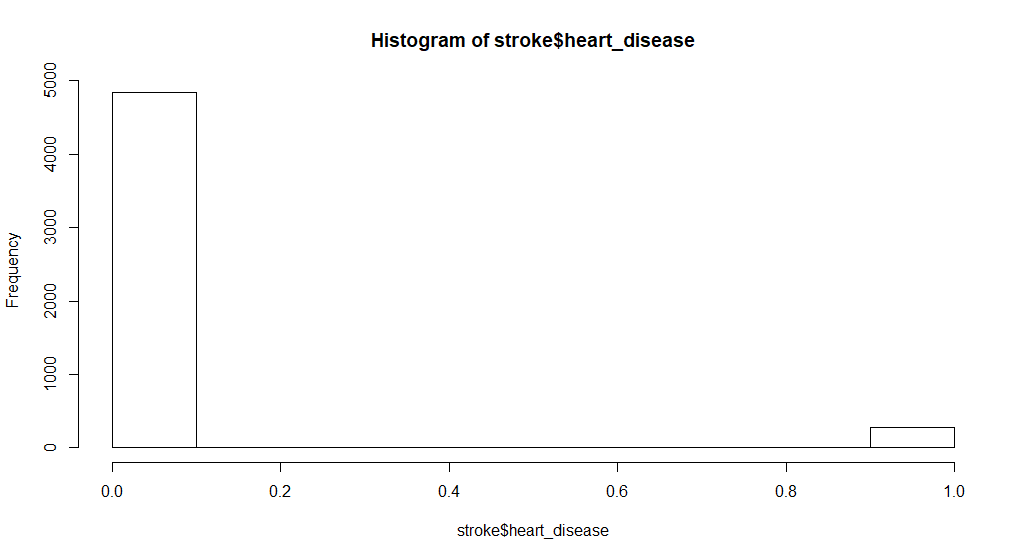
\includegraphics[scale=.5]{stroke-heart}    
\end{enumerate}

\pagebreak
\printbibliography

\end{document}
